

\chapter[High-fidelity and comprehensive DMS framework]{A framework for comprehensive and high-fidelity Deep Mutational Scanning}

\section{Introduction}

Within coming decades, millions of people will have their genome sequenced. Unfortunately, we have limited ability to interpret personal genomes, each carrying 100-400 rare missense variants~\cite{the_1000_genomes_project_consortium_global_2015} of which many must currently be classified as “variants of uncertain significance”. For example, gene panel sequencing aimed at identifying germline cancer risk variants in families yielded VUS for the majority of missense variants~\cite{maxwell_evaluation_2016}.  While functional variants can be predicted via computational tools such as PolyPhen-2\cite{adzhubei_method_2010} and PROVEAN~\cite{choi_fast_2012}, these methods can confidently detect only one third as many disease variants as are detectable by experimental assays~\cite{sun_extended_2016}. Unfortunately, experimental assays are either unavailable or economically inviable for most human disease genes. The development of Deep Mutational Scanning (DMS)~\cite{fowler_high-resolution_2010} is making it possible to produce maps that predict the functional impact of a large fraction of substitutions for at least a subset of residue positions. Recently, Starita and colleagues carried out a DMS screen for the critical RING domain of BRCA18~\cite{starita_massively_2015}. Despite this progress, no experimental sequence-function map has yet demonstrated high-accuracy scoring of the functional impact of all possible substitutions for any full length protein (see Table~\ref{table:DMSstudies}). Thus, the goal of complete, highly accurate DMS maps for full-length proteins remains undemonstrated.

Functional complementation can measure the ability of a mutant human protein to rescue the loss of the wild type enzyme (or its ortholog in the case of trans-species complementation)9,10. We have previously found that cell-based functional complementation assays facilitated highly accurate identification of disease variation across a diverse collection of human disease genes5. 

Here we describe a modular DMS framework to generate maps of variant function. The framework employs a novel mutagenesis strategy, functional complementation, two alternative sequencing-based selection screens, and a machine learning strategy that completes the map via imputation and regularization. We first evaluate our framework on the SUMO E2 conjugase UBE2I.

\section{Results}

To carry out deep mutational scans of protein sequences yielding comprehensive atlases of sequence-function relationships, we found it useful to organize the process into six stages (see Figure 1A): 1) mutagenesis; 2) generation of a clone library; 3) selection for clones encoding a functional protein; 4) read-out of the selection results and analysis to produce an initial sequence-function map; 5) computational analysis to impute missing values; and 6) computational analysis to refine measured values based on imputation models. This framework incorporates previously-described deep mutational scanning concepts as well as new experimental components (e.g., our saturation codon mutagenesis strategy) and analytic methods.  The last two stages enabling a complete and accurate DMS map have not been applied in any published DMS study.

We first describe a variant of the framework called DMS-BarSeq and apply it to the human SUMO conjugase UBE2I, exhaustively measuring the ability of protein variants to function and to physically interact with protein partners.  Next, we describe a more efficient DMS-TileSeq variant of the framework, and apply this to UBE2I.  Having combined these maps, we computationally infer missing data points and refine map quality.

\subsection{A barcode-based Deep Mutational Scanning strategy}

As an initial test of the overall framework, we first aimed to generate a map of functional missnse variation for UBE2I. For Stage 1 of the DMS framework---mutagenesis---we wished to achieve a relatively even representation of all possible single amino acid substitutions.  Furthermore, we wished to allow multiple mutations per clone, both because this could allow for greater mutational coverage for any given library size, and because it would offer an opportunity to discover intragenic epistatic relationships between variants.  To fulfill these requirements, we developed a mutagenesis protocol (Precision Oligo-Pool based Code Alteration or POPCode) which generates random codon replacements. POPCode scales up a previously-described technique11 in which oligonucleotides carrying a central 3-base degenerate region are hybridized to a uracil-containing wild-type DNA template, with completion of the mutant strand via non-displacing DNA polymerase extension and ligation, followed by degradation of the wild-type template.  To accomplish mutagenesis across the entire coding region, we designed a tiled collection of oligos (one per codon) and applied POPCode to generate a codon-mutagenized amplicon library for UBE2I.  In parallel, we carried out PCR with oxidized nucleotides 12 to enable deeper representation of amino acid changes achievable from single-nucleotide changes.

For Stage 2 of the framework---generation of a clone library---we employed an en masse recombinational cloning strategy to generate a Gateway Entry vector library of UBE2I variants (see Online Methods). This library was then transferred via en masse recombinational subcloning into a pool of randomly-barcoded plasmids enabling expression of UBE2I variants in yeast. The full-length sequence and barcode of each clone was established using a novel sequencing method called kiloSEQ which combines plate-position-specific index sequences with Illumina sequencing to carry out full-length sequencing for thousands of samples (see Online Methods). Based on sequence information, we retained clones that carried at least one amino acid substitution to generate a final library comprised of 6,553 UBE2I variants, covering different combinations of 1,848 (61\% of all possible) unique amino acid changes. Variant plasmids were pooled, together with empty vector and wild type control plasmids (see Online Methods).

For Stage 3, the selection of clones encoding a functional protein, we employed a previously described S. cerevisiae functional complementation assay5,13. This assay is based a yeast strain carrying a temperature sensitive (ts) allele of the UBE2I orthologue UBC9, and on the observation that human UBE2I rescues growth at an otherwise lethal elevated temperature.  Despite a billion years of divergence, yeast functional complementation assays of human disease genes can accurately discriminate pathogenic from non-pathogenic variants5,13.  The plasmid library from Stage 3 was introduced into the appropriate ts strain by en-masse transformation. Pools were then grown over a period of 48 hours at the permissive (25\celsius ) and selective (37\celsius ) temperatures, respectively (see Online Methods).

To read out the results of the selection (Stage 4), barcodes were sequenced at multiple timepoints to enable reconstruction of individual growth curves and normalized fitness quantification for each of the 6,553 strains. Functional complementation scores were calibrated so that a value of 0 corresponds to the mean fitness of the empty-vector control and a value of 1 corresponds to the average of wild type controls (see Online Methods). Each of the stages will be discussed in further detail below.



\subsubsection{POPCode: A Precision Oligo Pool Codon alteration mutagenesis method}

This method scales up a previously described method developed by Seyfang et al.11. To achieve complete wide coverage over the complete spectrum of possible amino acid changes we design oligonucleotides centering on each codon in the Open Reading Frame (ORF) of interest and replacing the target with a NNK degeneracy code. This has been previously demonstrated to allow all amino acid changes while reducing the chance of generating stop codons36 . 

When finding a set of suitable oligonucleotide sequences, two important criteria need to be considered: 
1) The melting temperature across the complete set is as uniform as possible as this will ensure a more even mutation rate across the ORF sequence; 2) the degenerate codon sequence should be located as close to the center of the oligo as permissible given the first criterium. To simplify the process of choosing an appropriate set of oligos based on these criteria I developed a web tool that can be used to calculate the optimal solution to the given problem. The tool merely requires the sequence of the target ORF and flanking vector sequences, a desired average oligo length and a maximum offset parameter. The offset parameter determines how many bases can be maximally added or removed from each side of a given oligo to optimize its melting temperature. 

In some cases a moderate deviation from the average in melting temperature for some oligos cannot be avoided. To alleviate these effects, the webtool also offers a mutation rate prediction. This is based on observations from all the POPCode procedures performed as part of this work in combination with linear regression. The prediction can be used to preemptivly adjust concentrations of potentially troublesome oligos in the POPCode protocol. An additional webtool feature based on the mutation rate prediction is the automatic calculation of necessary library size to achieve a desired mutational coverage. The webtool as available at \verb|http://llama.mshri.on.ca/cgi/popcodeSuite/main|.

%%Figure: PopCode schema

\begin{figure}[h!]
	\centering
	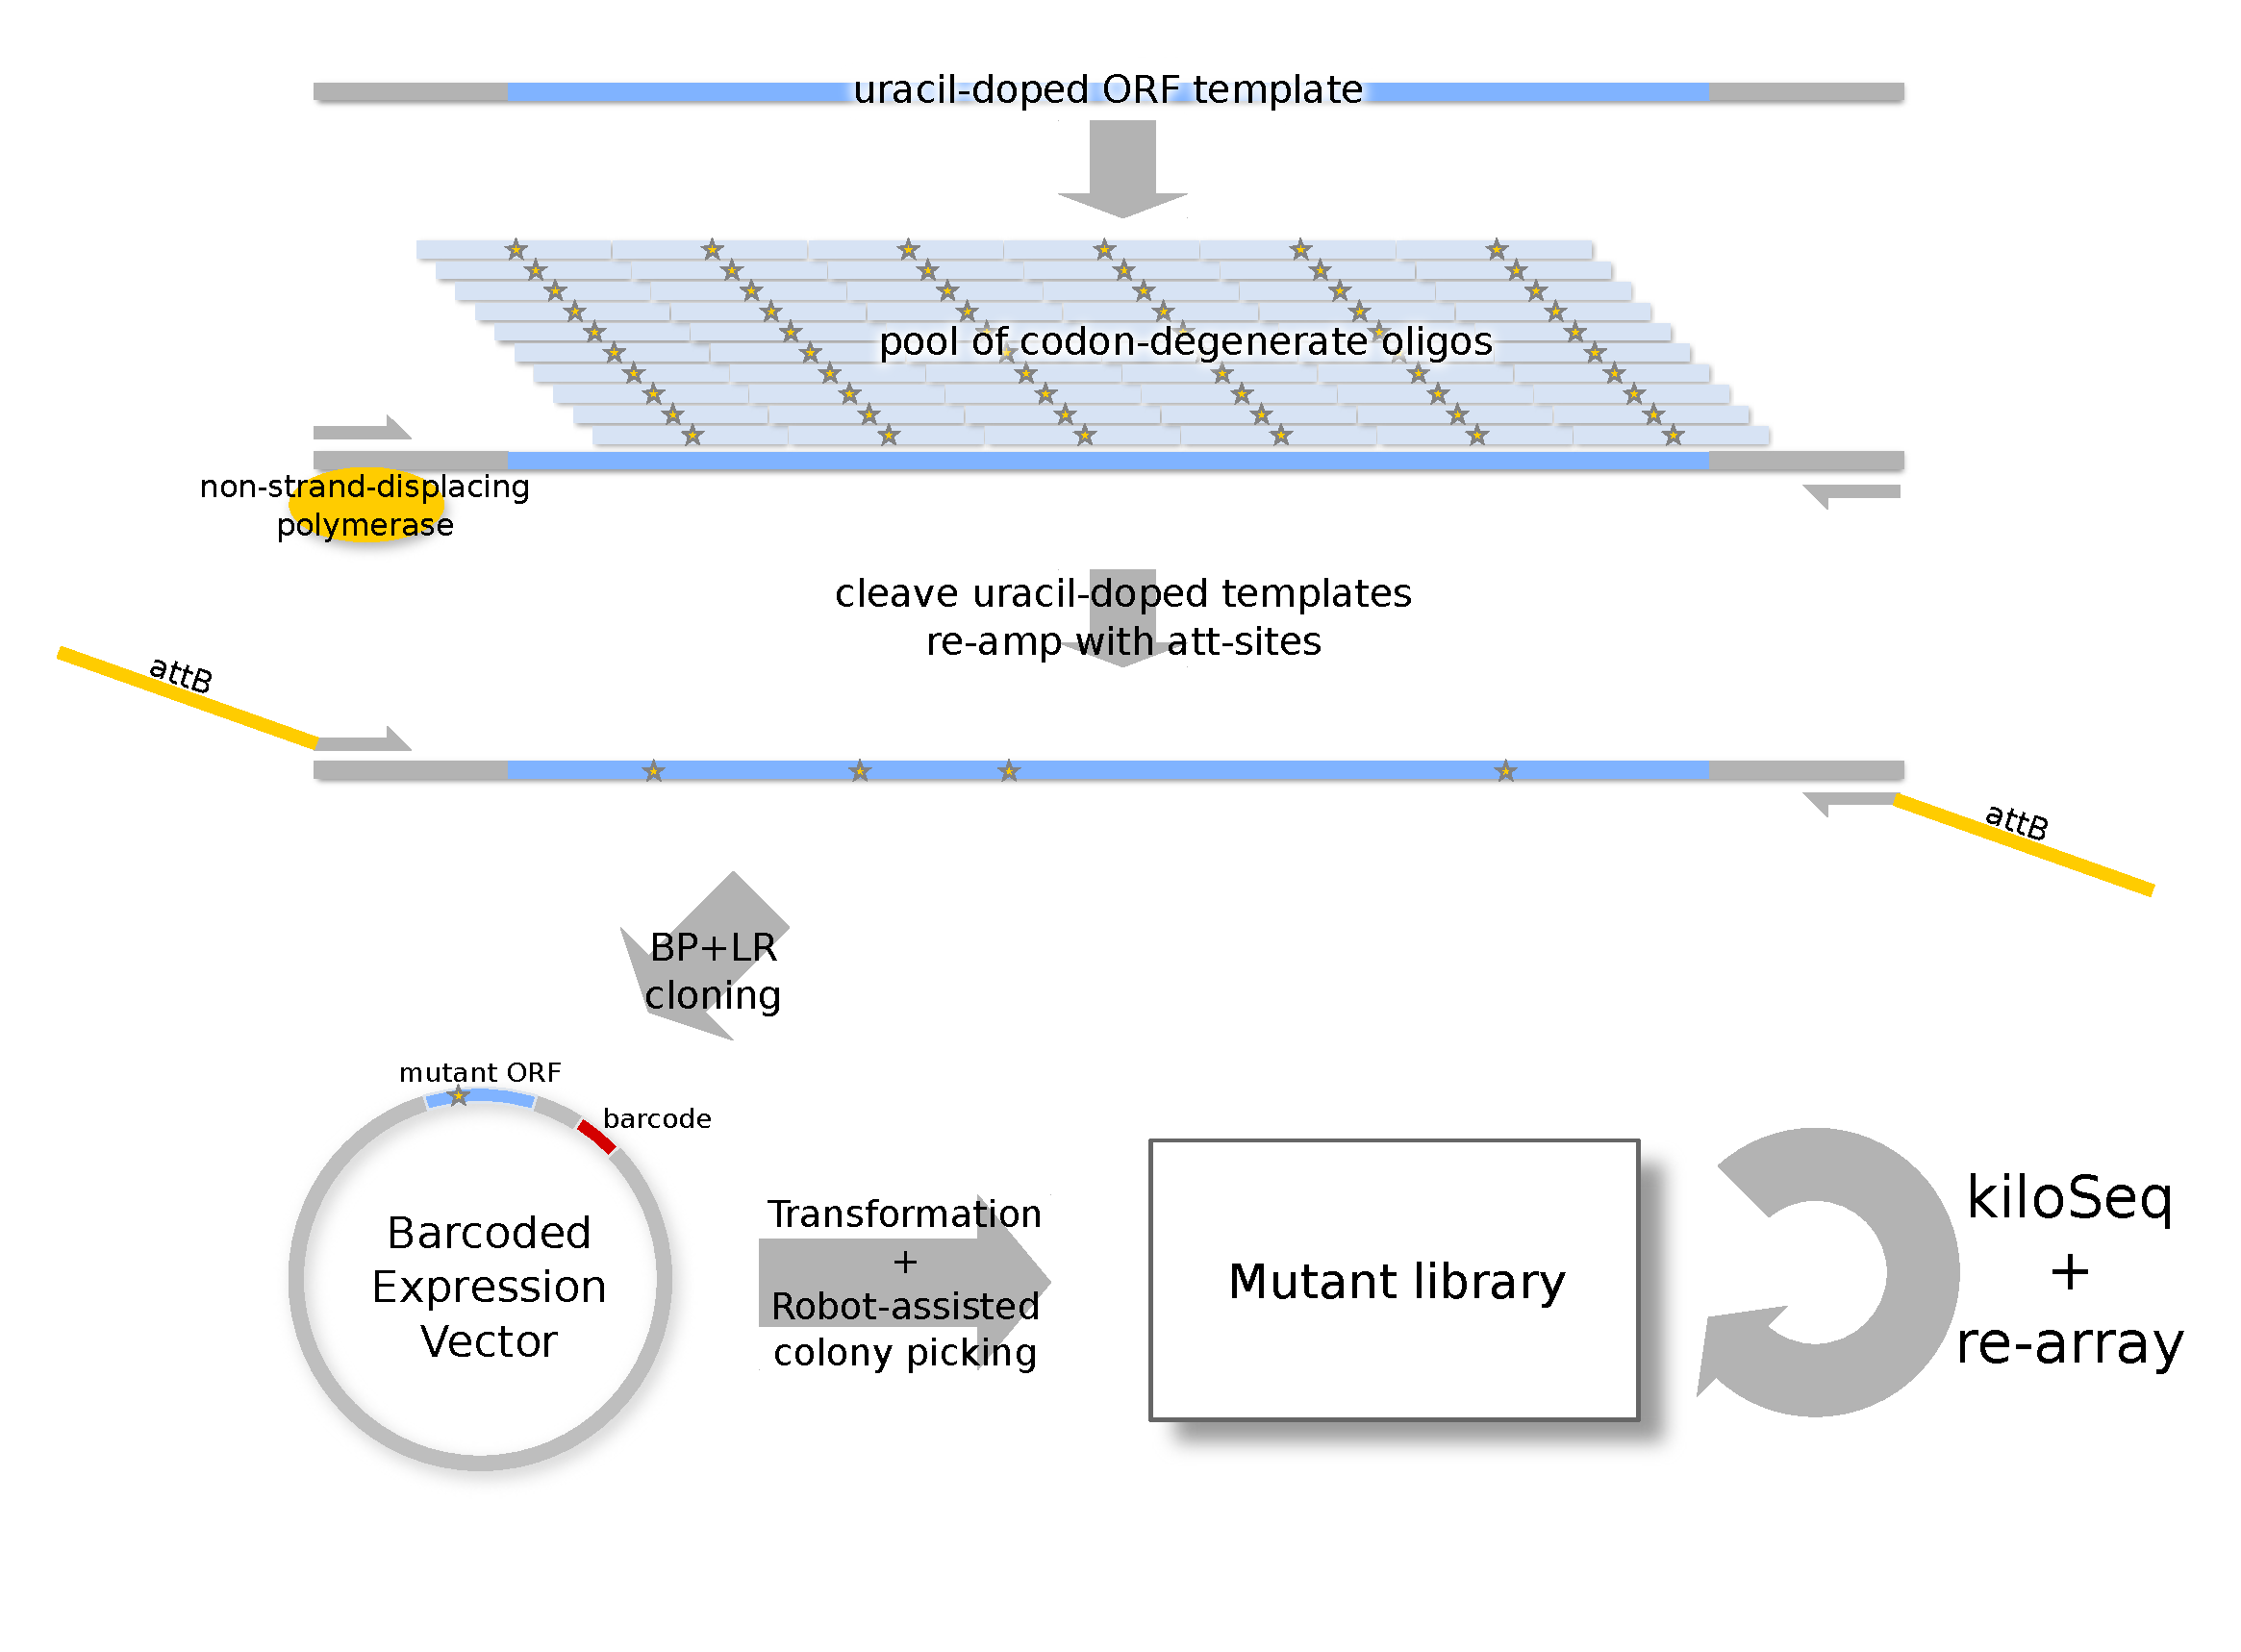
\includegraphics[width=\textwidth]{img/popcode_schema.pdf}%TODO: should be direct BP-LR cloning
	\caption{POPCode mutagenesis and library generation. A pool of codon-denerate oligos is hybridized to a uracil-doped template, gaps between oligos are closed via non-strand-displacing polymerase and the backbone sealed. Uracil-doped template is degraded to enrich for mutants. After mutagenesis, Gateway attB sites are added, followed by BP+LR cloning into barcoded vectors and transformation into bacteria. Finally, colonies are picked and arrayed.}
	\label{fig:popcode_schema}
\end{figure}


In the next step, the ORF sequence is PCR amplified in the presence of dUTP to generate uracil-doped template for the mutagenesis reaction. Oligonucleotide pools were then hybridized with the template. Gaps between hybridizations were filled and sealed with the non-strand-displacing Sulpholobus Polymerase IV. Following cleanup, the uracil-doped template was incapacitated using Uracil-DNA-Glycosylase (UDG). The mutagenesis product was then amplified with primers that added attB sites to allow Gateway BP cloning into entry vectors.

\subsubsection{KiloSEQ: A highly multiplexed amiplicon sequencing method}

To establish the identity of each plasmid barcode and its associated set of mutations in the target ORF we used kiloSEQ, which was developed in collaboration with SeqWell Inc., Boston. The complementation vector is designed such that the variant ORF and the barcode locus are in close proximity to each other, so that only a relatively small segment of the plasmid needs to be amplified for sequencing. The primers used in these reactions contain well-specific tags allowing each well on each plate to be uniquely identified. In the next step, Nextera tagmentation using Tn5 transposase is used to break the amplicons into random fragments and simultaneously ligate them to Illumina sequencing linkers with plate-specific indices. We then re-amplify the pool with  3'-specific primers, to enrich for fragments that contain the well tags. The resulting library is now ready for paired-end sequencing. In each pair of reads, one read will contain the well tag and the barcode locus, whereas the other will contain a fragment of the mutant ORF.
%TODO: move to methods: This is done using a hydrocycler, allowing for thousands of PCR reactions to be performed in parallel. ----- Amplicons can then be plate-wise pooled.

\begin{figure}[h!]
	\centering
	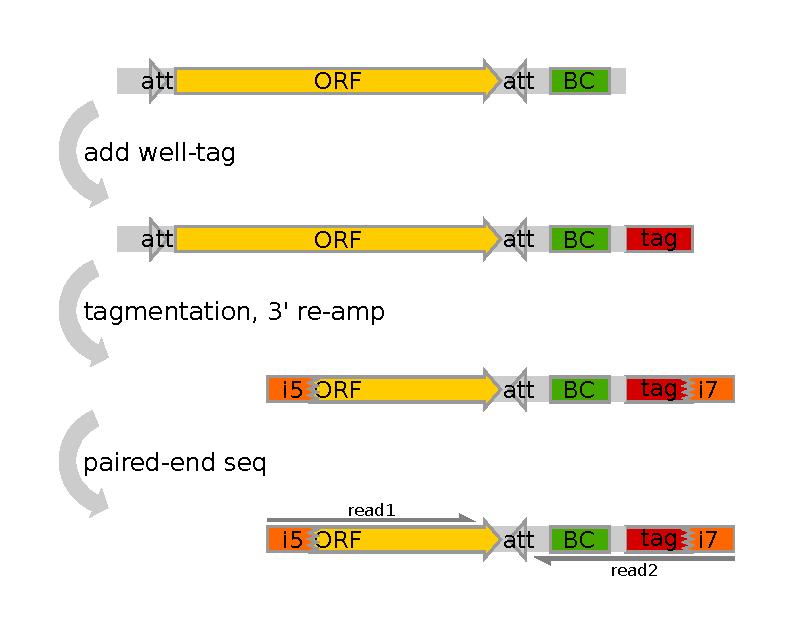
\includegraphics[width=.5\textwidth]{img/kiloseq_schema_new.pdf}
	\caption{KiloSEQ schema. 1) For each library well, amplicons containing the variant ORF (gold) and Barcode locus (green) are amplified with primers adding a well-specific tag. 2) Tn5 tagmentation fragments the DNA while simultaneously adding Illumina i5/i7 linkers. 3' re-amplification enriches for fragments containing the well tags. 3) Each pair of sequencing reads now contains a fragment of ORF sequence and the associated barcode and well tag.}
	\label{fig:kiloseq_schema}
\end{figure}

To process the results of a KiloSEQ sequencing run, a special software pipeline was developed, which can be divided into three phases: Demultiplexing; Barcode clustering; and Alignment and variant calling.
The first phase---demultiplexing---takes place on two levels, corresponding to library plates and the wells within those plates. The plate level of demultiplexing is automatically performed by Illumina's bcl2fastq software, which resolves i5-i7 index combinations. The second phase is performed on a high performance computing cluster. Sets of read pairs are distributed across computing nodes, where they are processed by worker scripts. The well-tag within each R2 read is identified using a k-mer search algorithm, and read-pairs are sorted accordingly into bins. Each bin corresponds to one well in a given plate. At the same time, barcode sequences are extracted from the R2 reads in preparation for the next phase. 

The second phase---barcode clustering---uses the extracted barcode sequences within each bin and clusters them according to their Levenstein distance (i.e. the number of edit operations separating them). This step is necessary due to resolve possible contamination across wells that occurred during library preparation. Each barcode cluster corresponds to a different clone, and the concrete sequences within each clusters to different sequencing errors. The the most frequent sequence within each cluster is interpreted as the true barcode. Finally, read pairs within each bin are again subdivided according to their respective barcode cluster.

The third phase---alignment and variant calling---is then executed for each barcode cluter within each well within each plate. The R1 reads are aligned to the template sequence and variants are called. This is complicated by the fact that KiloSEQ library preparation usually creates a certain amount of cross-contamination between wells. While single or multi-nucleotide variants are still relatively unproblematic to identify, standard tools were unable to identify copy number variations (CNVs) due to these problems. We thus developed a custom method for CNV detection, based on detecting sudden changes in read depth across the alignments. First the read depth is normalized to the average read depth across the plate. Then a one-dimensional Sobel operator is used to detect sharp edges in the signal. An example of this can be seen in Figure~\ref{fig:border_detect}.

\begin{figure}[h!]
	\centering
	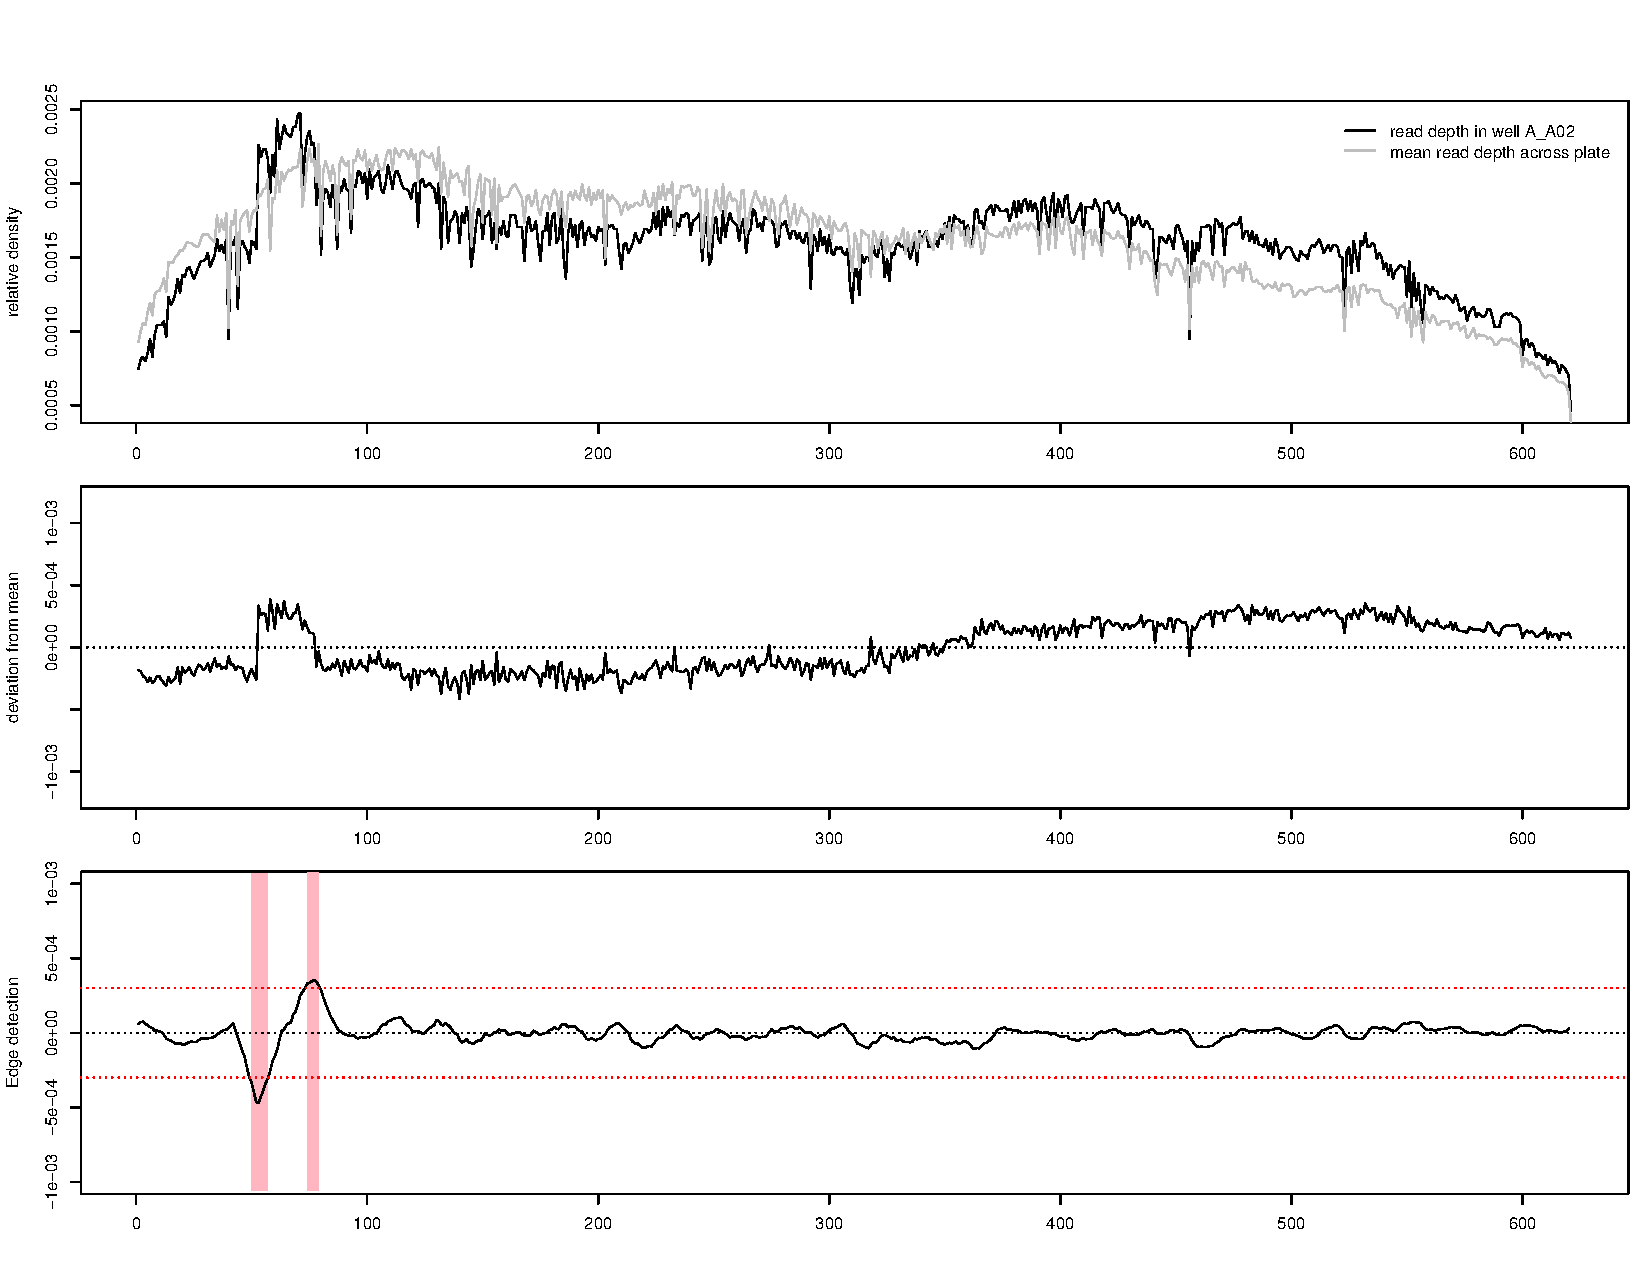
\includegraphics[width=\textwidth]{img/border_detect.pdf}
	\caption{Indel detection example. A duplication event in well \texttt{A\_A02} is detected by normalizing relative read depth by the mean depth across the plate and using a Sobel operator to detect sudden changes.}
	\label{fig:border_detect}
\end{figure}


After successful genotyping with kiloseq, we determined the subset of clones that (i) contained a minimum of one missense mutation, (ii) did not contain any insertions or deletions, (iii) did not contain mutations outside of the ORF, (iii) had unique barcodes, (iv) had sufficient read coverage during kiloSEQ to allow for confident genotyping.
Over half of clones in the library conformed to these criteria. The single largest reason for exlusion was the occurrence of indels and CNVs (Figure~\ref{fig:popcode_census}A). 

An analysis of the mutation signatures across clones generated by POPCode revealed that two different mechanisms appear to underly the mutagenesis. When considering only mutations that change more than one base in a given codon, there is an equal chance for every possible base, except in the third position in which almost no adenine or cytosines were placed. This is consistent with the NNK degeneracy code present in the POPCode oligos. By contrast, variants that change only a single base in a given codon show a strong bias for transitions over transversions. These could be introduced due to polymerase error (Figure~\ref{fig:popcode_census}B). This is also reflected in the relative share of single nucleotide variants, which make up 56\% of mutations (Figure~\ref{fig:popcode_census}C). As a consequence, when examining the mutation coverage across the sequence of the ORF, it is clearly visible that the share of amino acids reachable with a single nucleotide change from the respective wildtype codon is much closer to saturation than the the set of all possible amino acid changes (Figure~\ref{fig:popcode_census}D). Additionally some hotspots are visible, in which mutation rate is higher, which is likely due to different hybridization efficiencies of oligos across the ORF sequence.

Using the Biomatrix robot, we re-arrayed the subset of usable clones into a condensed final library of 40 plates.


%%Figure library coverage, census, and bias map

\begin{figure}[h!]
	\centering
	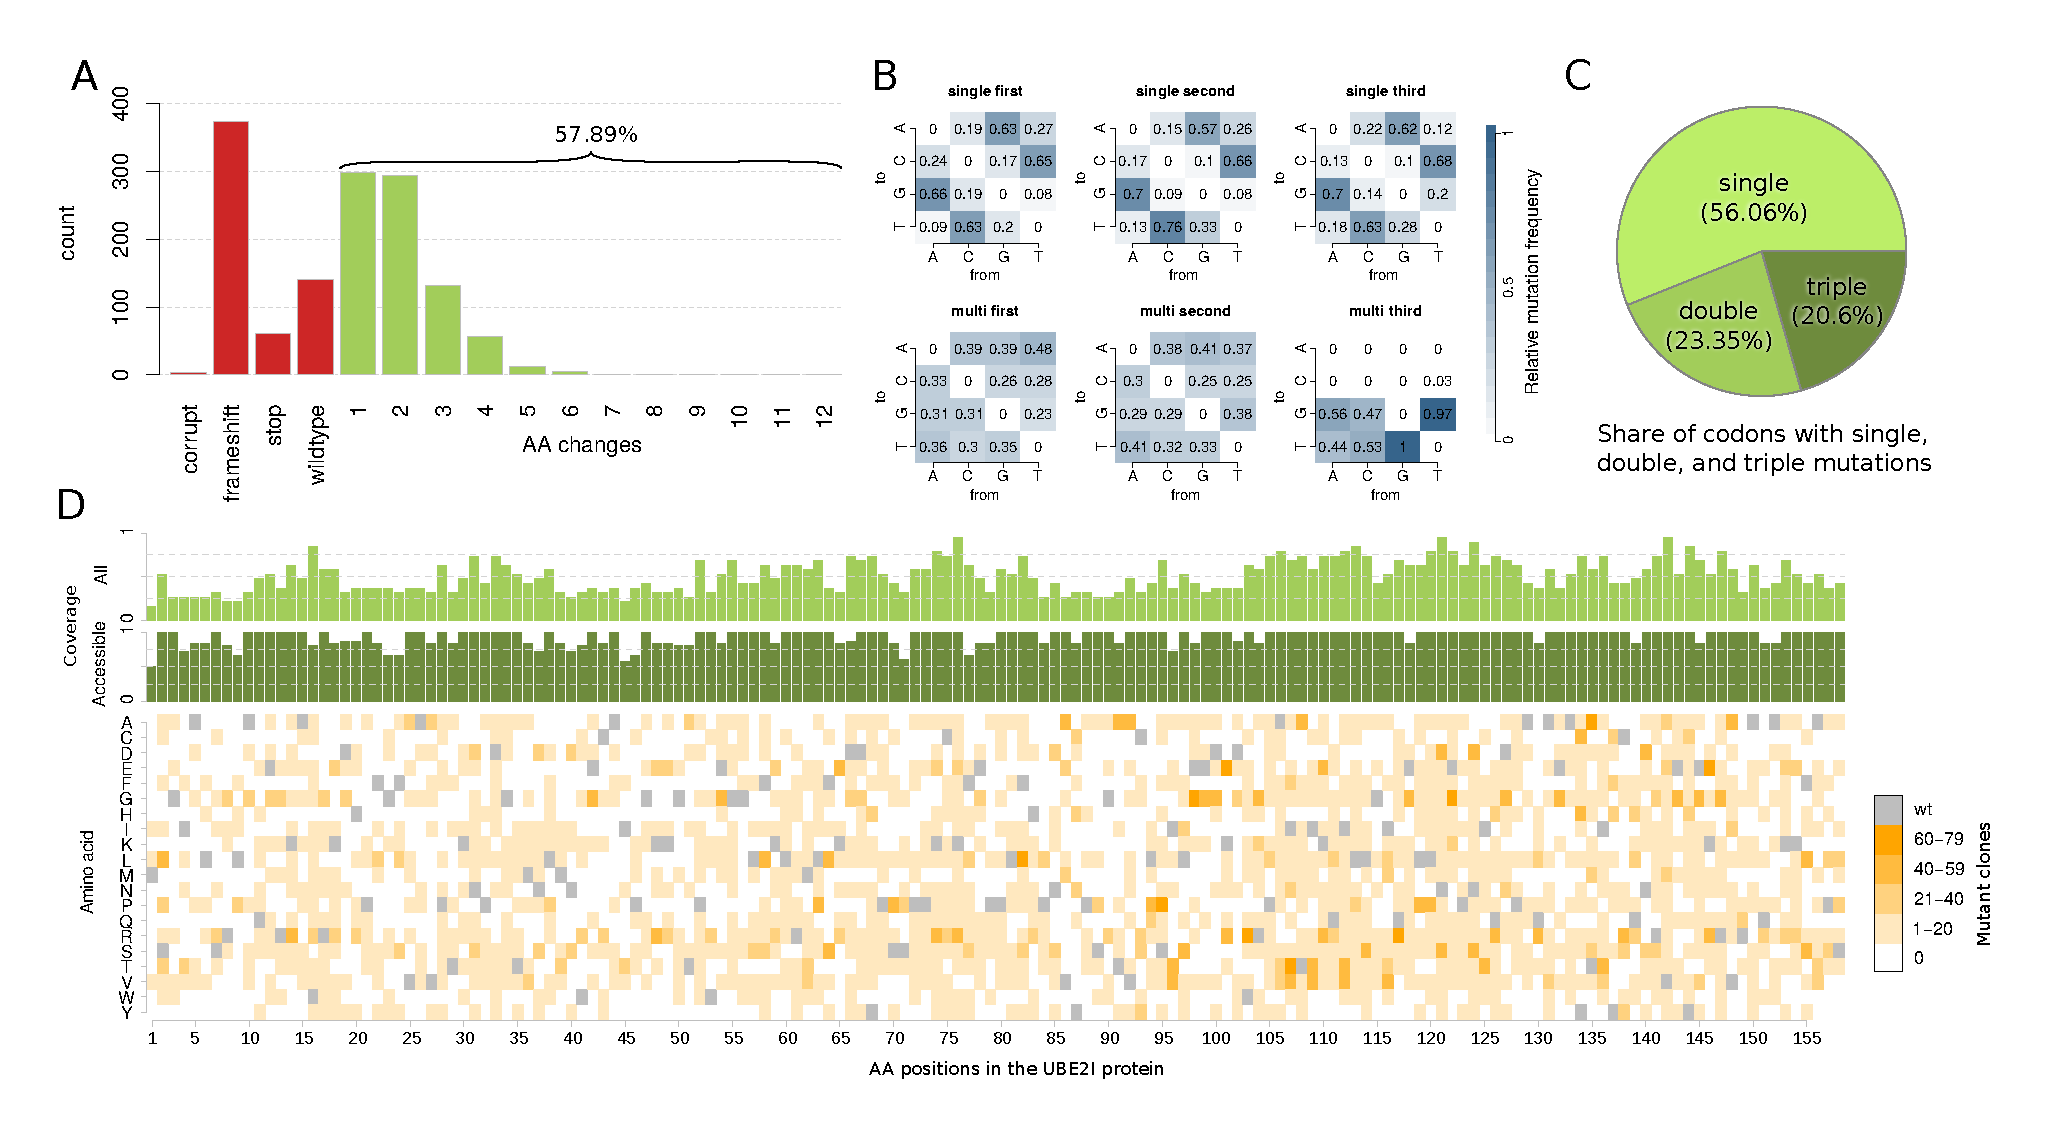
\includegraphics[width=\textwidth]{img/popcode_census.pdf}
	\caption{KiloSEQ census of UBE2I POPCode library. A) Breakdown of KiloSEQ results for a set of five 384 well plates of mutant clones generated by POPCode. Corrupt: Clones containing mutations outside of the ORF; Frameshift: Clones containing indels or copy number variants; Stop: Clones containing stop codons. B) Breakdown of mutations in codons. Top: Single nucleotide variants; Bottom: Multi-nucleotide variants. Columns correspond to the first, second and third position in a codon. C) Relative shares of single, double and triple nucleotide variants among all missense variants in the library. D) Coverage map of missense variants in the library. Light green track: Coverage across all possible amino acids; Dark green track: Coverage across amino acids reachable with a single nucleotide change from the wildtype codon.}
	\label{fig:popcode_census}
\end{figure}


\subsubsection{A barcoded-based functional map of UBE2I}

To assess the quality of complementation scores before further refinement in Stages 5 and 6, we first examined reproducibility of scores between technical replicates (Figure 1B, top panel), and biological replicates (different clones carrying the same mutation; Figure 1B, bottom panel).  In each case the scores were reproducible (Pearson’s R of 0.97 and 0.78, respectively).   To further examine score quality, we carried out semi-quantitative manual complementation spotting assays for a subset of mutants that spanned the range of fitness scores (see Supplementary Methods). Complementation scores from deep mutational scanning correlated well with these small-scale tests. Indeed, agreement between the large-scale and manual scores was about the same as agreement between internal replicates of the large-scale scores (Figure 1B,C). 

As a further ‘sanity check’, we next examined evolutionary conservation and common predictors of deleteriousness, such as PolyPhen-23 and PROVEAN4.  Although these do not perfectly predict the functionality of amino acid changes5 —and may be particularly ill-suited for assessing amino acid changes that require multiple nucleotide substitutions in a given codon—they should nonetheless correlate with functionality.  Indeed, DMS-BarSeq fitness scores were significantly correlated with evolutionary conservation and PolyPhen-2 and PROVEAN scores (Figure 1D top panel, Supplementary Figure S1). Finally, we confirmed that, as expected, amino acid residues on the protein surface are more tolerant to mutation than those in the protein core or within interaction interfaces (Figure 1D, bottom panel).  Taken together, these observations support the biological relevance of the DMS-BarSeq approach.

\subsection{A complete functional map of UBE2I}

\subsubsection{An alternative strategy for DMS via tiled regional sequencing}

While the DMS-BarSeq approach has many advantages (see Discussion), its performance comes at the cost of producing and maintaining an arrayed clone library, and of determining the full-length sequence of each coding region and barcode for each clone. We therefore investigated an alternative approach called DMS-TileSeq: Instead of tracking the fitness of each individual clone, we carried out en masse measurements of the frequency of each variant in the pool before and after selection, by deep sequencing.  Sequencing was carried out for a set of short amplicon tiles that collectively encompass the complete coding region.  In this way, we can discern the impact of each mutation by observing the impact of selection on the abundance of clones carrying this mutation.

In terms of mutagenesis (Stage 1), DMS-TileSeq is identical to DMS-BarSeq.  Given the mutagenized amplicon library, the cloning step (Stage 2) was carried out by en masse recombinational subcloning into complementation vectors (thus skipping the step of arraying and sequencing individual clones).  This plasmid pool was next transformed en masse into the ubc9-ts strain appropriate for assessing the complementation ability of UBE2I variants. As with DMS-BarSeq, DMS-TileSeq employs pooled strains grown competitively (Stage 3) at the permissive and selective temperatures. However, instead of using barcode sequencing to determine the fitness associated with individual stains, we directly sequence the coding region from the clone population to determine the frequency of each variant in each pool (before and after selection). To overcome the problem of distinguishing mutations from sequencing errors, we divide the coding region into tiles such that each individual template molecule can be completely sequenced on both strands.  By requiring that each variant be seen on both strands, the incidence of base-calling errors can be substantially reduced6.  DMS-TileSeq requires that the library be sufficiently complex to ensure that the effect of a mutation is determined from enough clones and over enough genetic backgrounds (where there are multiple variants per clone) to be reproducible (see Online Methods).

To validate the reliability of DMS-TileSeq, we first applied it to UBE2I and compared the results with those obtained using DMS-BarSeq. Correlation between DMS-TileSeq and DMS-BarSeq was comparable to the correlation observed between biological replicates of DMS-BarSeq (Supplementary Figure 2), suggesting that reproducibility of DMS-TileSeq is at least comparable to that of DMS-BarSeq. DMS-TileSeq and DMS-BarSeq showed comparable agreement with complementation scores from manual assays (Supplementary Figure 3).  Thus, DMS-TileSeq avoids the substantial cost of arraying and sequencing thousands of individual clones, while performing on par with DMS-BarSeq in terms of reliability of the functional complementation scores it produces.


\subsubsection{Imputation and regularization of missing or less accurate data}

Having performed two independent deep mutational scans of UBE2I using functional complementation assays, we wished to integrate both results into a single comprehensive high-quality map. To accomplish this, we first combined the results of each screening approach into a joint map.  This required bringing the maps onto the same scale. Using a regression-based transformation function, we transformed the DMS-TileSeq scores to the more intuitive scale of DMS-BarSeq (where 0 corresponds to the typical score of a null mutant and 1 corresponds to the typical score of a wildtype control). We then combined scores from the two methods, giving greater weight to more confident measurements (see Online Methods).

As is the case for all previously published DMS maps, our combined map contained some entries that were poorly measured or missing (e.g., because these substitutions were underrepresented in the input clone library). To fill in the gaps, we trained a machine learning model to impute missing data (Stage 5 of our framework). Specifically, we trained a random forest regression model on a set of biochemical and structural features, as well as features intrinsic to our dataset (for example, the average score of well-measured substitutions at a given position). This procedure also allowed incorporation of information from clones in DMS-BarSeq that had multiple mutations, through the use of two features: 1) the average score of all clones carrying the mutation of interest, and 2) the average corrected score from clones that carry the mutation of interest, where the correction makes use of a multiplicative fitness model to remove the fitness effect of other mutations present (see Supplementary Methods). We assessed performance of the imputation model using cross-validation and found that the root-mean squared deviation of imputed values is on par with measurement error in experimentally measured data (Supplementary Figure S3).

To improve the accuracy of entries for which the experimental measurements were least confident, we employed a regularization method (Stage 6 of the framework).  This was achieved by combining experimental measurements and imputed values, weighting by the estimated accuracy of each (see Methods). The complete refined functional map of UBE2I after imputation and regularization can be seen in Figure 2A. 

To evaluate the complete map, we applied manual functional complementation assays to a set of variants that were chosen to represent the full range of fitness scores.  DMS fitness scores corresponded closely with manual functional complementation assays (Supplementary Figure S4A), validating our framework.  To more specifically evaluate the imputation process, we selected a smaller test set of variants (again spanning the range of impact scores), and recalculated imputation scores after excluding variants in the test set from the training process.  Imputed scores not only corresponded closely with measured DMS scores, but also with the results of manual complementation assays (Supplementary Figure S4B).  Collectively, our framework yielded a comprehensive map covering all possible missense variants, with overall quality that was on par with the highest-quality measurements from either screen alone.


\subsection{Evaluation and validation of the UBE2I map}

\section{Methods}

\section{Discussion}

